%%%%%%%%%%%%%%%%%%%%%%%%%%%%%%%%%%%%%%%%%%%%%%%%%%%%%%%%%%%%%%%%%%%
%
% First comes an example EPS file -- just ignore it and
% proceed on the \documentclass line
% your LaTeX will extract the file if required
\begin{filecontents*}{example.eps}
%!PS-Adobe-3.0 EPSF-3.0
%%BoundingBox: 19 19 221 221
%%CreationDate: Mon Sep 29 1997
%%Creator: programmed by hand (JK)
%%EndComments
gsave
newpath
  20 20 moveto
  20 220 lineto
  220 220 lineto
  220 20 lineto
closepath
2 setlinewidth
gsave
  .4 setgray fill
grestore
stroke
grestore
\end{filecontents*}
%
\RequirePackage{fix-cm}
%
%\documentclass{svjour3}                     % onecolumn (standard format)
%\documentclass[smallcondensed]{svjour3}     % onecolumn (ditto)
\documentclass[smallextended]{svjour3}       % onecolumn (second format)
%\documentclass[twocolumn]{svjour3}          % twocolumn
%
\smartqed  % flush right qed marks, e.g. at end of proof
%
%\usepackage{graphicx,natbib}
\usepackage{graphicx}
%
% \usepackage{mathptmx}      % use Times fonts if available on your TeX system
%
% insert here the call for the packages your document requires
%\usepackage{latexsym}
% etc.
%
% please place your own definitions here and don't use \def but
\newcommand{\mnras}{MNRAS}
\newcommand{\nat}{Nature}
\newcommand{\aap}{A\&A}
\newcommand{\apj}{ApJ}
\newcommand{\apjl}{ApJL}
\newcommand{\physrep}{Phys.Rep.}
\newcommand{\prd}{Phys.Rev.D}
\newcommand{\araa}{ARA\&A}
\newcommand{\DDT}{D$_{\Delta{\rm t}}$}
%
% Insert the name of "your journal" with
% \journalname{myjournal}
%
%%%%%%%%%%%%%%%%%%%%%%%%%%%%%%%%%%%%%%%%%%%%%%%%%%%%%%%%%%%%%%%%%%%

\begin{document}

\title{Time delay cosmography%\thanks{Grants or other notes
%about the article that should go on the front page should be
%placed here. General acknowledgments should be placed at the end of the article.}
}
%\subtitle{Time delay cosmography}

\titlerunning{Time delay lens cosmography}        % if too long for running head

\author{Tommaso Treu         \and
        Philip J. Marshall %etc.
}

%\authorrunning{Treu \& Marshall} % if too long for running head

\institute{Tommaso~Treu \at
Department of Physics and Astronomy, \\
University of California,\\
Los Angeles, CA 90095, USA\\
\email{tt@astro.ucla.edu}           %  \\
%             \emph{Present address:} of F. Author  %  if needed
           \and
Philip~J.~Marshall \at
Kavli Institute for Particle Astrophysics and Cosmology, \\
P.O. Box 20450, MS29, \\
Stanford, CA 94309, USA \\
}

\date{Received: date / Accepted: date}
% The correct dates will be entered by the editor

\maketitle

%%%%%%%%%%%%%%%%%%%%%%%%%%%%%%%%%%%%%%%%%%%%%%%%%%%%%%%%%%%%%%%%%%%

\begin{abstract}

Here goes the abstract. mention blindness

\keywords{First keyword \and Second keyword \and More}
% \PACS{PACS code1 \and PACS code2 \and more}
% \subclass{MSC code1 \and MSC code2 \and more}

\end{abstract}

%%%%%%%%%%%%%%%%%%%%%%%%%%%%%%%%%%%%%%%%%%%%%%%%%%%%%%%%%%%%%%%%%%%

\section{Introduction [TT]}
\label{sec:intro}

% % % % % % % % % % % % % % % % % % % % % % % % % % % % % % % % % %

The measurement of cosmic distances is central to our understanding of
cosmography, i.e. the description of the geometry and kinematics of
the universe. The discovery of the period luminosity relation for
Cepheids led to the realization that the universe is much bigger than
the Milky Way and that it is currently expanding. Relative distance
measurements based on supernova Ia light curves were the turning point
in the discovery of the acceleration of the universe
\citep{Riess:1998p21184,Per++99}.

In the two decades since the discovery of the acceleration of the
universe, distance measurements have improved steadily. For example,
the Hubble constant has now been measured to 2.4\% precision
\citep{Rie++16} while the distance to the last scattering surface of
the cosmic microwave backgrond is now known to approximately 0.5\%
precision \citep[depending on the assumed cosmological
model]{WMAP9,Pla15}. This precision is more than sufficient for all
purposes related to our understanding of phenomena occurring within
the universe, like galaxy evolution.

In spite of all this progress, the most fundamental question still
remains unanswered. What is causing the acceleration? Is this {\it
dark energy} something akin to Einstein's cosmological constant or is
it a dynamical component? Answering this question from an empirical
standpoint will require further improvements in the precision of
distance measurements \citep{Suy++12,Wei++13,Kim++15,Rie++16}.  In
practice, measuring the dark energy equation of state requires an
accurate model of the scale parameter of the universe as a function of
time, particularly when dark energy is dynamically most relevant,
i.e. below $z\sim1$.

%\begin{figure}[!t]
%\begin{center}
%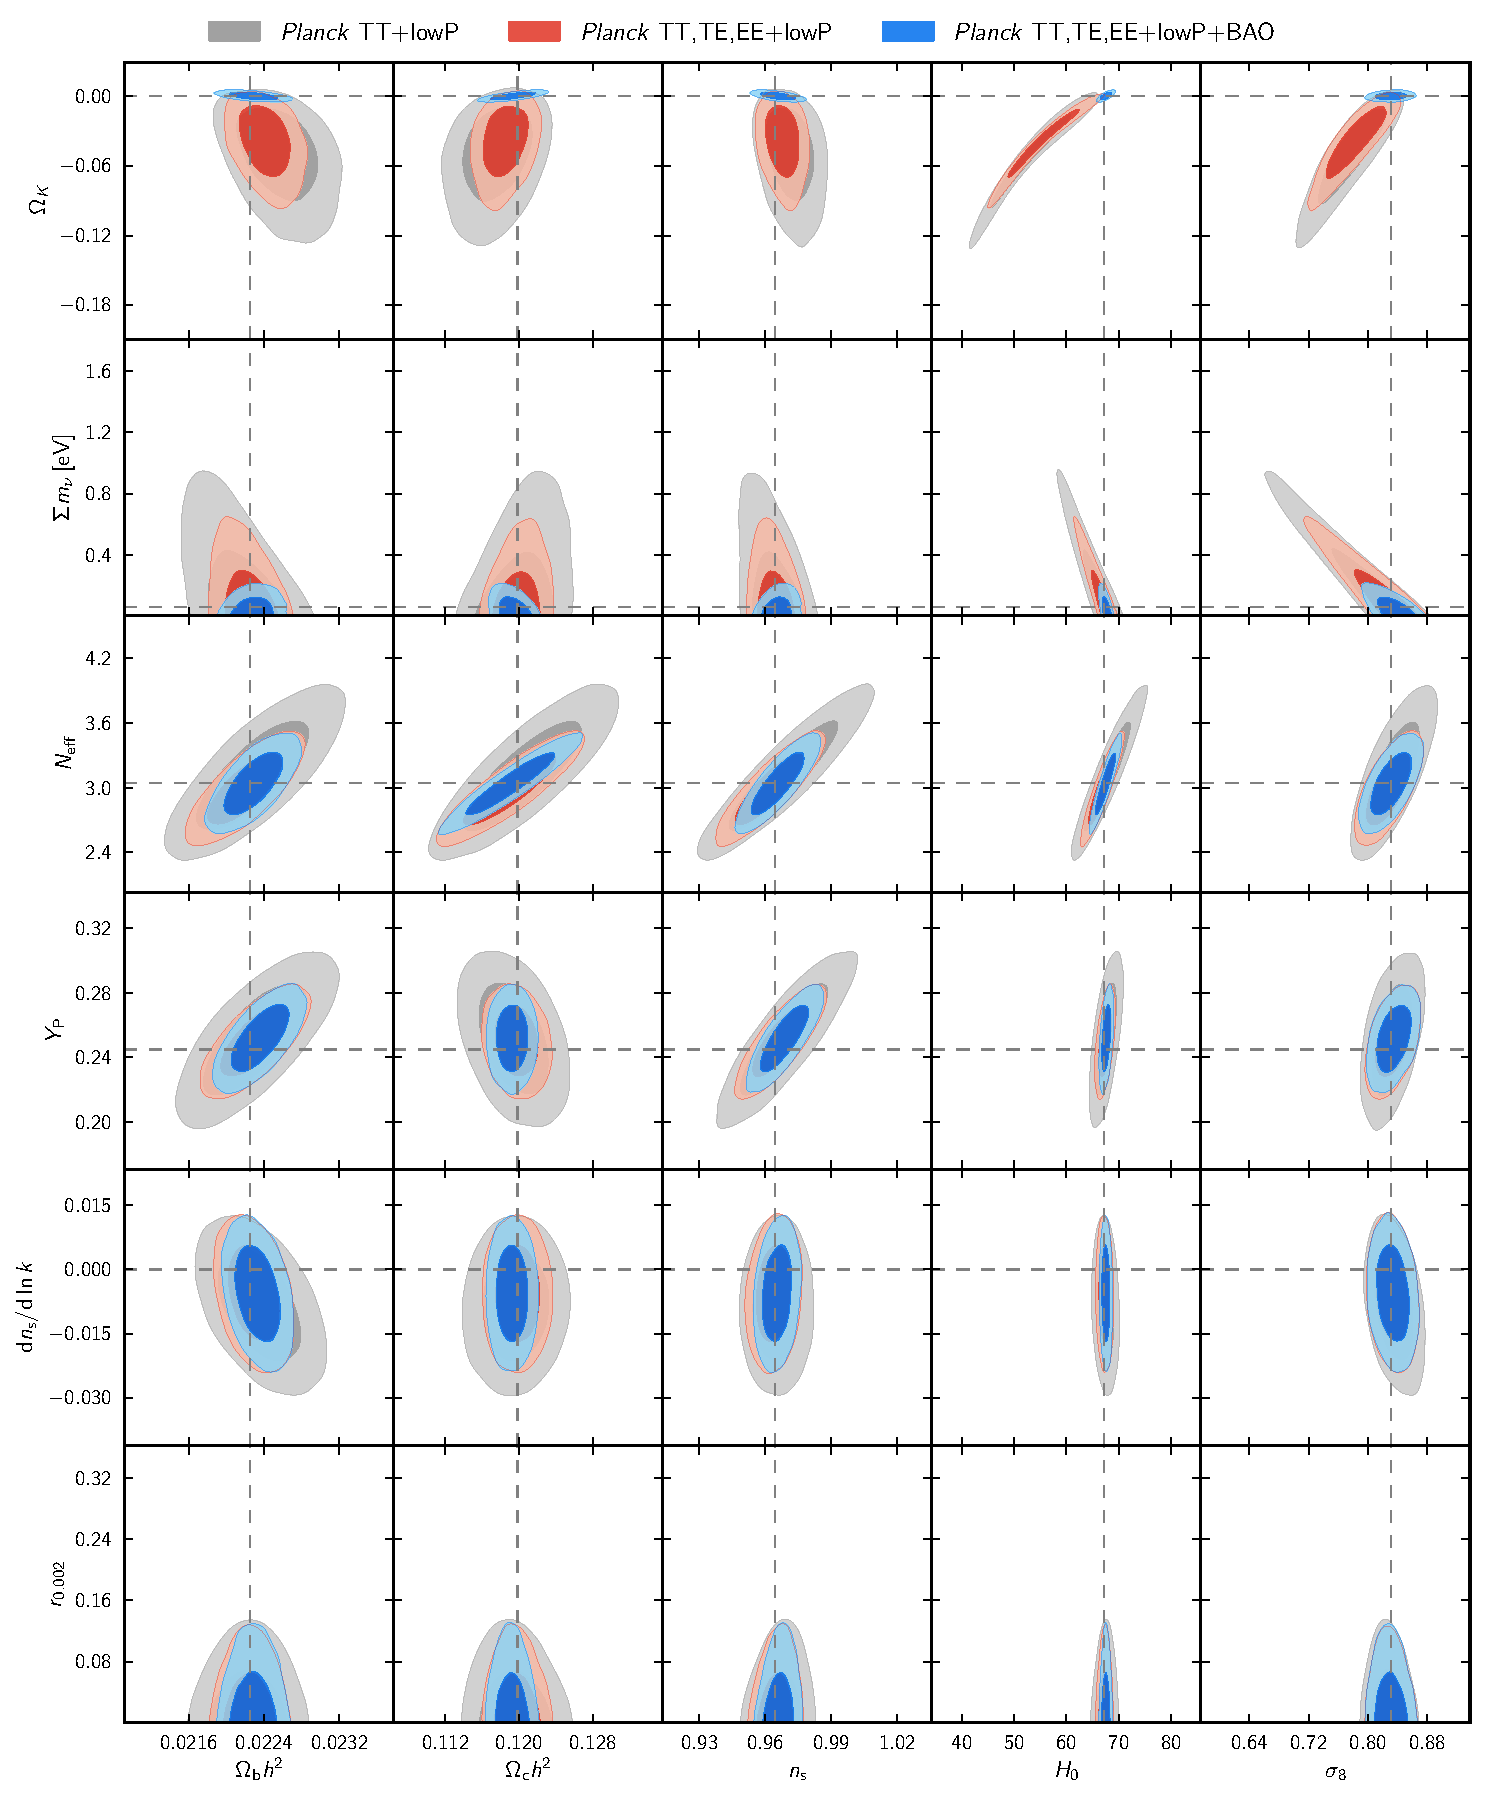
\includegraphics[width=0.5\textwidth]{figures/grid_1paramext.pdf}
%\caption{The figure, taken from \cite{Pla15}, shows the confidence
%intervals obtained for 1-parameter extension of the basic $\Lambda$CDM
%model obtained using Plank measurements themselves, and in combination
%with baryonic acoustic oscillations. Note that the interpretation of
%CMB data long is strongly degenerate, even in these simple
%models. Lower redshift distance measurements, in case from BAO, break
%the degeneracies. See the original paper \cite{Pla15} for details
%about the figure and input parameters.}
%\label{fig:CMB}
%\end{center}
%\end{figure}

Cosmic microwave background anisotropies primarily provide a
measurement of the angular distance to the last scattering surface,
obtain by comparing the angular scale of the acoustic peaks with the
baryonic acoustic oscillation scale. Therefore, the constraints set by
CMB anisotropy data on dark energy parametere are highly degenerate in
a generic cosmological model
\citep[e.g.,][]{Pla15}. Breaking the degeneracy requires strong
assumptions about the universe (e.g., flatness or dark energy being
the cosmological constant), or lower redshift distance
measurements. Many dedicated experiments are currently under way or
being planned with this goal in mind.

%A summary of distance
%measurements with approximate precision and redshift range is given in
%Figure~\ref{fig:comparedist}.
%[Include distance ladder, CMB, BAO, cosmic clocks, fgas]

%\begin{figure}[!t]
%\begin{center}
%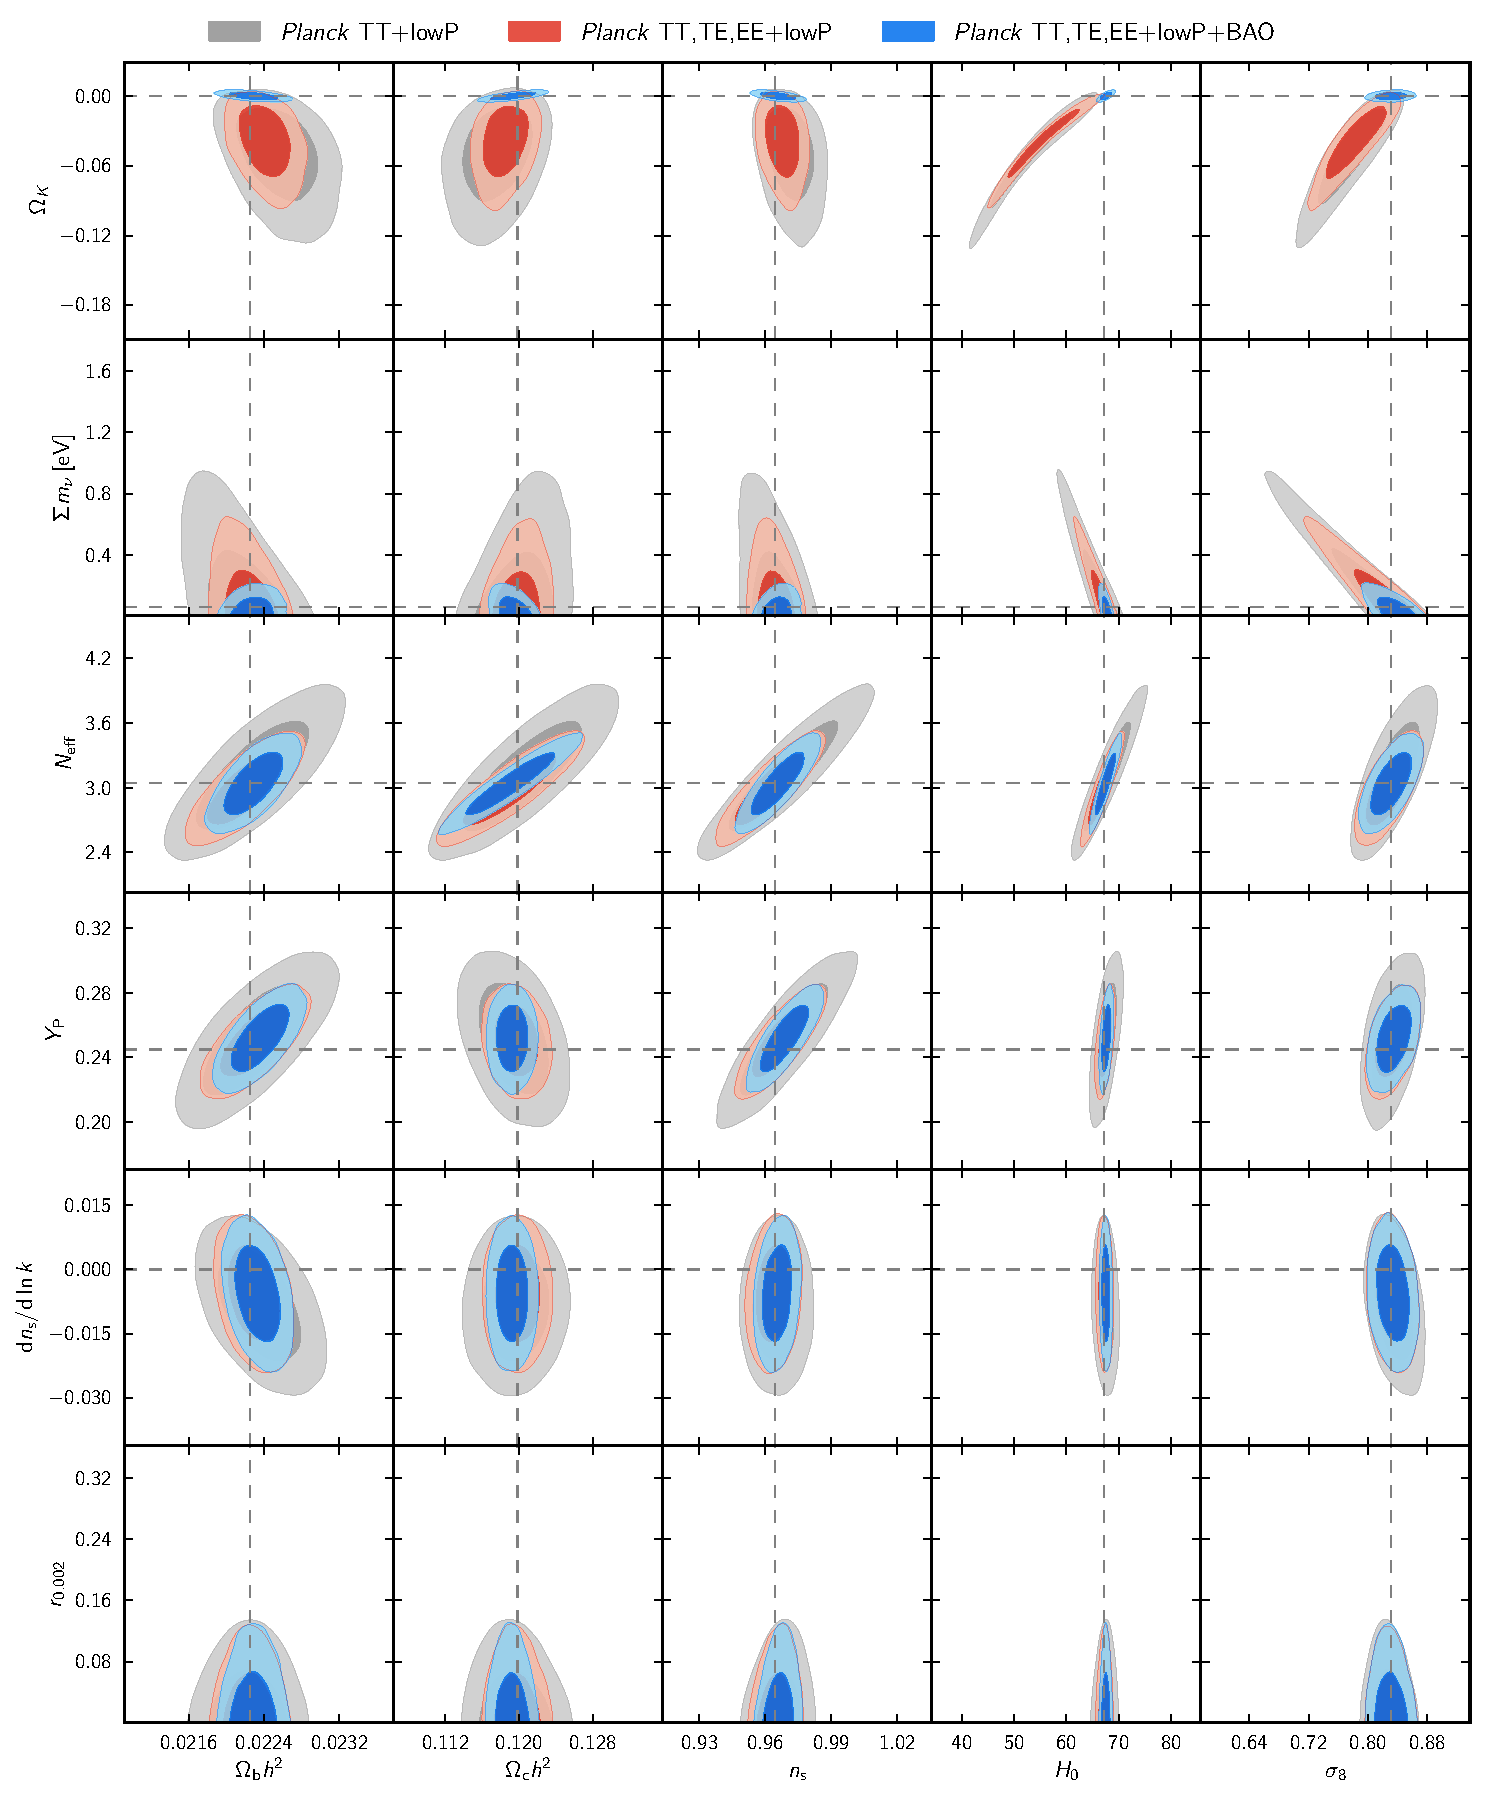
\includegraphics[width=0.5\textwidth]{figures/grid_1paramext.pdf}
%\caption{Summary of current distance measurements}
%\label{fig:comparedist}
%\end{center}
%\end{figure}

Precision, however, is not sufficient by itself. In addition to
controlling the known statistical uncertainties ({\it precision}),
modern day experiments need to control systematic errors ({\it
accuracy}) in order to fullfill their potential, including the
infamous unknown unknowns. The most direct way to demonstrate accuracy
is to compare independent measurements that have comparable precision. An
interesting, currently topical, and relevant case is that of the 3$-\sigma$ tension
between the local distance ladder determination of H$_0$
\citep{Rie++16} and that inferred by the Plank satellite assuming a
flat $\Lambda$CDM model \citep{Pla15}. The tension could be due to an
unknown source of systematic errors in either or both of the two measurements, or
it could be indicative of new physics, for example an effective number of
relativistic species greater than three. Independent measurements with
comparable precision are the best way to make progress.
% For example,
% the WMAP9 measurement \citep{Cal++13} is significantly less in tension
% with the cosmic distance ladder data than the Planck one.
While independent measurements of the same phenomenon, or reanalysis of the
same data \citep{Efs14,SFH15}, are certainly useful and necessary,
completely independent datasets based on different physical phenomena
provide qualitatively new information.

Ideally, the comparison between independent measurements should be
carried out blindly, so as to minimize experimenter bias. Two mutually
blind measurements agreeing that the equation of state parameter $w$
is not $-1$ would be a very convincing demonstration that the dark
energy is not the cosmological constant. Conversely, the significant
disagreement of two blind and independent measurements, could be the
first sign of new physics.

In this review we focus on strong lensing gravitational time delays as
a tool for cosmography. As we shall see, this probe provides a direct
and elegant way to measure absolute distances out to cosmological
redshift. When the line of sight to a distant source of light is
suitably well aligned with an intervening massive system, multiple
images appear to the observer. The arrival time of the images depends
on the interplay of the geometric and gravitational delays specific to
the configuration. If the emission from the source is variable in
time, the difference in arrival time is measurable, and can be
interpreted via a so-called ``time delay distance'' $\Ddt$.
In the simplest case, this distance is just a multiplicative combination
of the three angular diameter distances between the observer, deflector and
source. $\Ddt$ is
inversely proportional to the Hubble Constant $H_0$, and more
weakly dependent on other cosmological parameters. As several authors
have pointed out \citep{Hu05,Lin11,Suy++12,Wei++13}, achieving
sub-percent precision and accuracy on the measurement of the Hubble
constant will be a powerful addition to Stage III and IV dark energy
experiments. The independence of time delays from other traditional
probes of cosmology, makes them very valuable for precise and accurate
cosmology. For example, time delays yield an {\it absolute}
measurement of distance without relying on Cepheids or any other local
rung of the distance ladder, and because the relevant quantities are
angular diameter distances rather then luminosity distances, the
approach is insensitive to dust or
other photometric errors.

This review is organized as follows. In Section~\ref{sec:intro} we
summarize the history of time delay cosmography up until the turn of
the millennium, in order to give a sense of the early challenges and
how they were overcome. In Section~\ref{sec:theory}, we review the
theoretical foundations of the method, in terms of the gravitational
optics version of Fermat's principle. In Section~\ref{sec:measurement}
we describe in some detail the elements of a modern time delay
distance measurement, emphasizing recent advances and remaining
challenges. In Section~\ref{sec:cosmo} we elucidate the connection
between time delay distance measurements and cosmological parameters,
discussing complementarity with other cosmological
probes. Section~\ref{sec:outlook} critically examines the future of
the method, discussing prospects for increasing the precision, testing
for accuracy, and synergy with other future probes of dark energy. A
brief summary is given in Section~\ref{sec:summary}.

Owing to space limitations, we could only present a selection of all
the beautiful work that has been published on this topic in the past
decades. We refer the readers to recent
\citep{Bar10,Ell10,Tre10,TMC12,Jackson:2013p30763,Jac15,T+E15}
and not-so-recent \citep{B+N92,CSS02,K+S04,Fal05,SKW06}
excellent reviews and textbooks \citep{SEF92} for additional
information and historical context.


\section{A brief history of time delay cosmography [TT]}
\label{sec:history}

\citet{Ref64} first suggested that strong lens time delays could be
used to measure absolute, cosmological distances, and
therefore the Hubble Constant to leading order. Unfortunately, no
strong lensing systems were known at that time, and therefore his
intuition remained purely theoretical for over a decade.

The prospects of using time delays for cosmography suddenly brightened
in the late seventies, with the discovery of the first strongly lensed
quasar \citep{WCW79}. Even though they were not the strongly lensed
supernovae that Refsdal had had in mind, quasar fluxes are sufficiently
variable \citep{Van82} that people were able to start to put Refsdal's
idea in practice \citep{Van89}.
The first multiply imaged supernova was discovered in 2014,
fifty years afer Refsdal's initial suggestion \citep{Kel++15}, lensed
by a foreground cluster of galaxies. The time delays are being
measured at the time of writing
\citep{Rod++16,Kel++16}; however, it is unclear at the moment whether the
cluster potential can be constrained with sufficient accuracy to
yield interesting cosmological information \citep{Tre++16}. In general,
we expect the more straightforwardly-modeled, more numerous
galaxy-scale time delay lenses to be the most useful systems for
cosmography, with supernovae competing for attention with quasars \citep{O+M10}.
In this review, we will restrict our case to the to date much more common and
better understood case of variable active galactic nuclei (AGN) being lensed by
foreground elliptical galaxies.

Discovery and monitoring of lensed quasars continued in the eighties and
nineties, powered by heroic efforts. By the end of the millennium the
number of known strongly lensed systems was in double digits
\citep{CSS02}, and the first truly robust time delays were measured
\citep{Kun++97,Sch++97}.
The industrial detection of multiply imaged AGN finally took off at the
beginning of the current millennium, with the improvement of panoramic
search technology in dedicated or existing surveys
\citep{Bro++03,Oguri:2006p5865,Agn++15}.

The initial period of time delay cosmography was marred by controversies over
systematic errors.  The measurement of time delays was particularly
controversial during the nineties as the quality of the early data
allowed for multiple estimated values \citep{PRH92}, owing to the combined
effects of gaps in the data, and microlensing noise in the optical
light curves. This problem was solved definitively at the turn of the
millennium, with the beginning of modern monitoring campaigns,
characterized by high cadence, high precision, and long duration, both
at optical and radio wavelengths
\citep{Fas++99,Fas++02,Bur++02,Eig++05}, as illustrated in
Figure~\ref{fig:oldvsmoderndt}. We discuss
modern monitoring campaigns in more detail in Section~\ref{ssec:timedelay}.

%%%%%%%%%%%%%%%%%%%%%%%%%%%%%%%%%%%%%%
\begin{figure*}
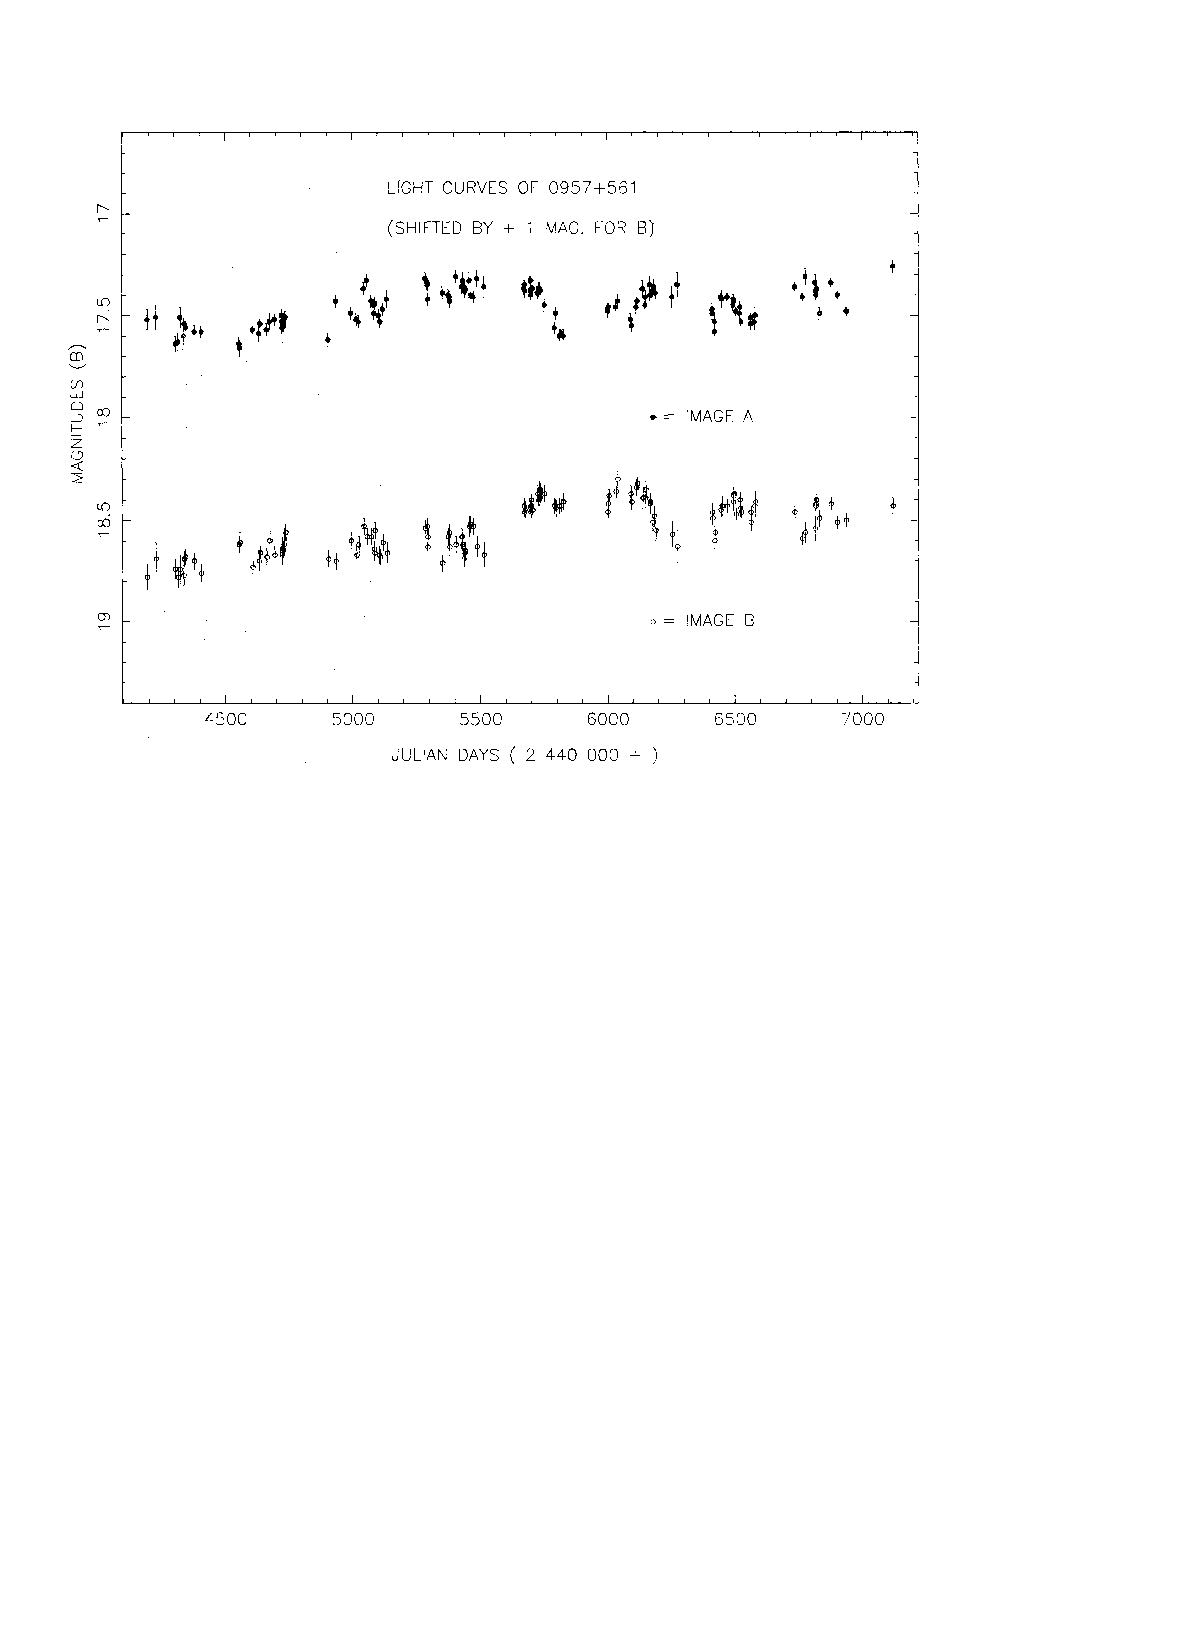
\includegraphics[width=0.48\textwidth]{figures/Vanderriest89_fig5.pdf}
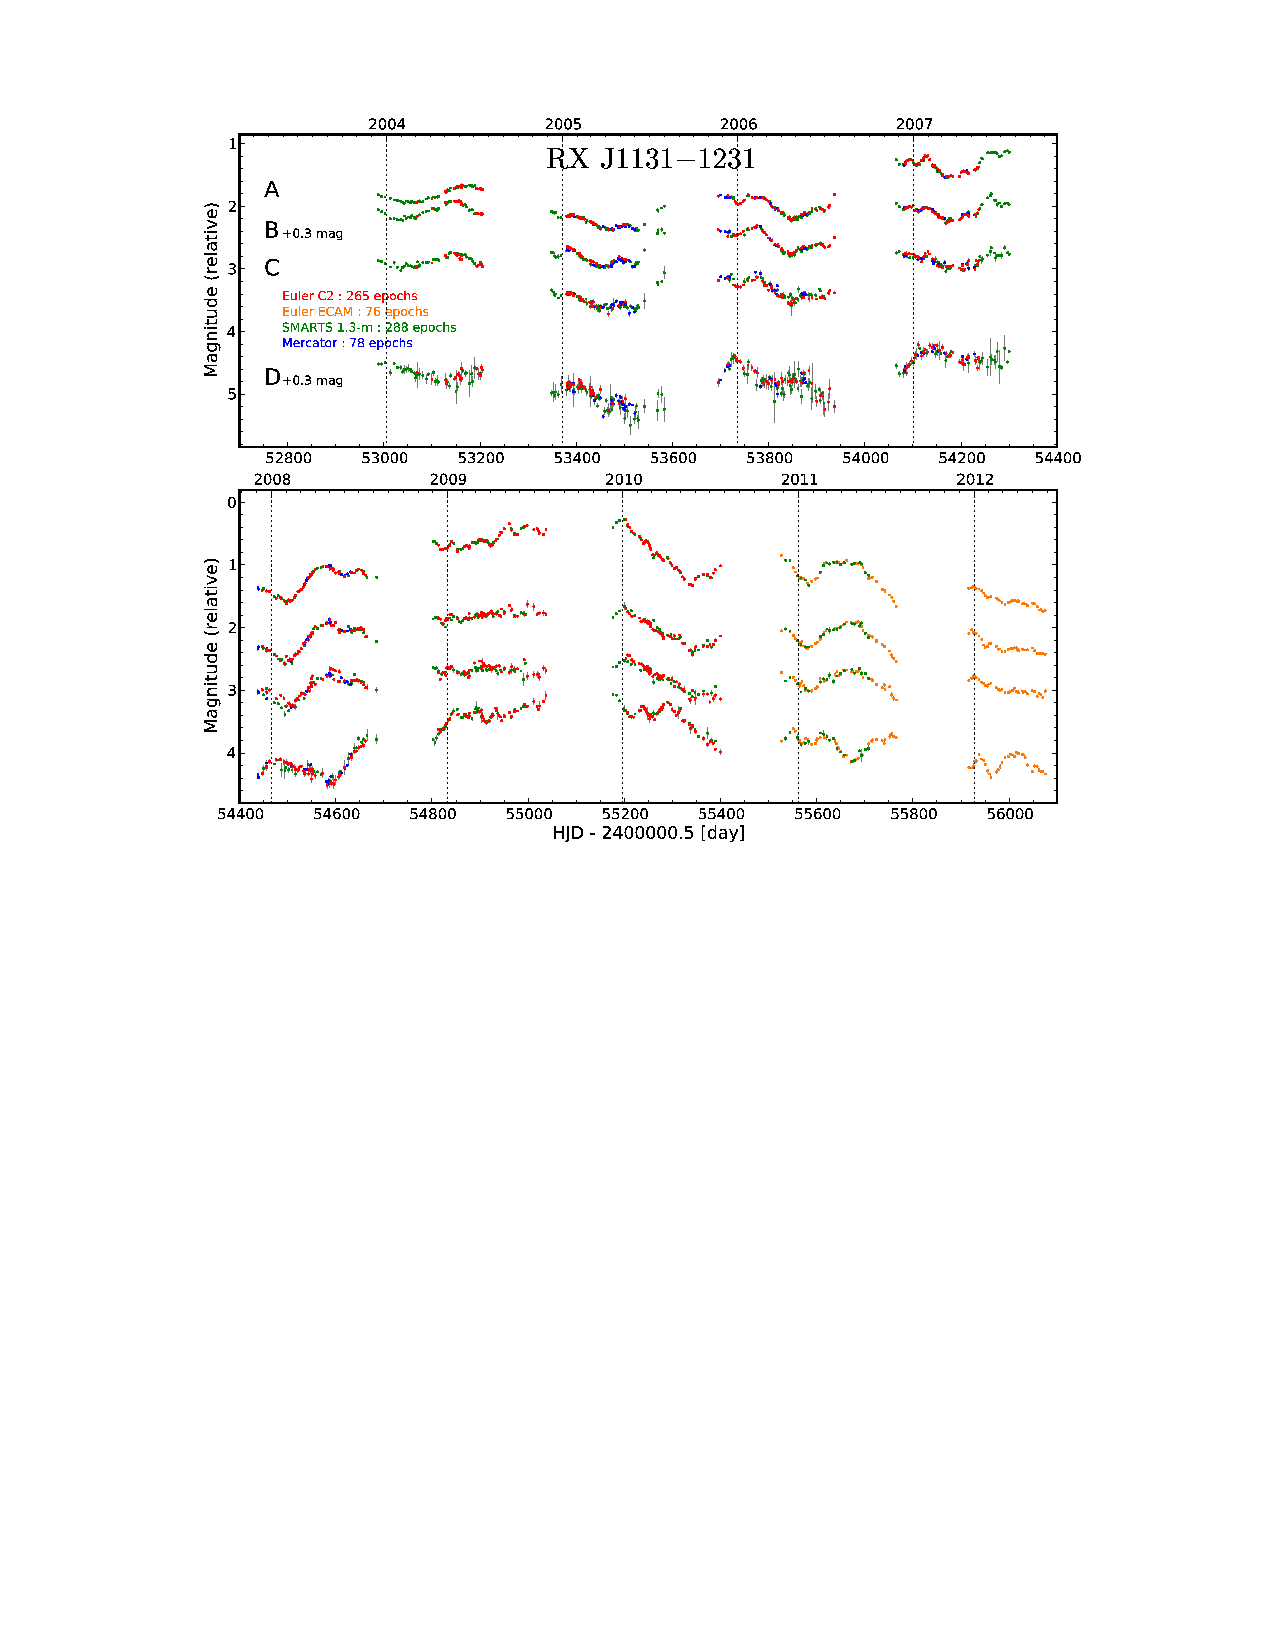
\includegraphics[width=0.48\textwidth]{figures/Tewes13-fig4.pdf}
\caption{Comparison between one of the early light curves \citep[left
panel, from][]{Van89}, and a modern light curve from COSMOGRAIL
\citep[right panel, from][]{Tew++13}. Note the improved photometric
precision, cadence, and duration of the light curves, allowing for
unambiguous determination of the time-delay to within 1-2\% precision.}
\label{fig:oldvsmoderndt}
\end{figure*}
%%%%%%%%%%%%%%%%%%%%%%%%%%%%%%%%%%%%%%

Finally, when robust time delays started to become available, the
focus of the controversy shifted to the modeling of the gravitational
potential of the lens. Typically, in the mid nineties, the only
constraints available to modelers were the quasar image positions and
to lesser extent flux ratios (limited by microlensing, variability and
differential extinction). Thus, the best one could do was to assume
some simple form for the lens mass distribution, such as a singular isothermal
sphere,
% thus breaking the mass sheet degeneracy,
and to neglect the
effects of structure along the line of sight. Given these necessary
but oversimplistic assumptions, random errors grossly underestimated
the total uncertainty, leading to measurements that were apparently
significantly inconsistent
between groups, or with those from other techniques
\citep{K+S04}. Since then, two methods have been pursued in order to
% break degeneracies in more flexible modeling of the lensing data and
obtain realistic estimates of the uncertainties. One consists of using
large samples of systems with relatively weak priors
\citep{Ogu07b}. The other method consists of obtaining high quality data for
each lens system, including detailed imaging of the quasar host galaxy
\citep{Keeton:2000p241,WBB04,Suy++06}, or non-lensing data like the deflector
stellar velocity dispersion \citep{T+K02b} and the properties of
galaxies along the line of sight \citep{K+Z04,Suy++10}. We discuss
these approaches in Section~\ref{ssec:lensmodel}. The astounding
improvement in data quality over the past two decades is illustrated
in Figure~\ref{fig:oldvsmodernimage}.

%%%%%%%%%%%%%%%%%%%%%%%%%%%%%%%%%%%%%%
\begin{figure*}
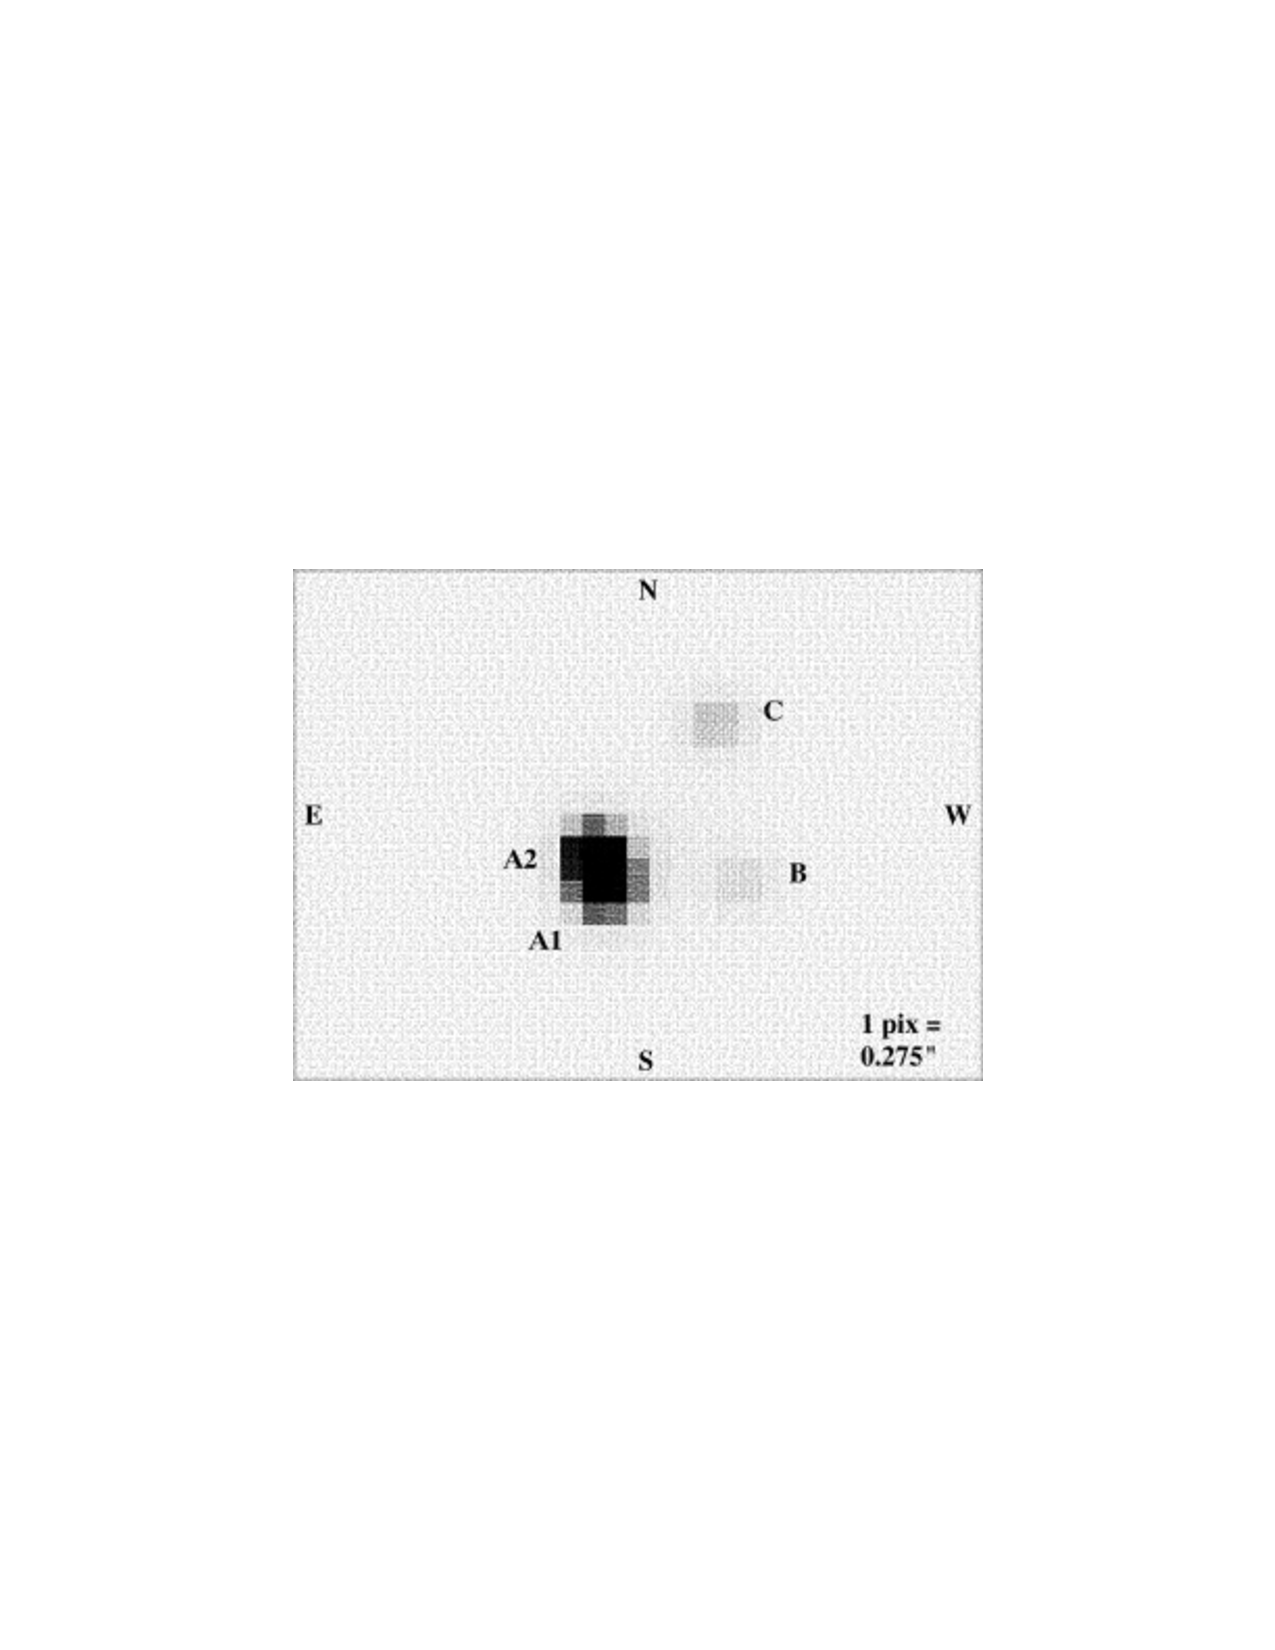
\includegraphics[height=3.5cm]{figures/Schechter97_fg1.pdf}
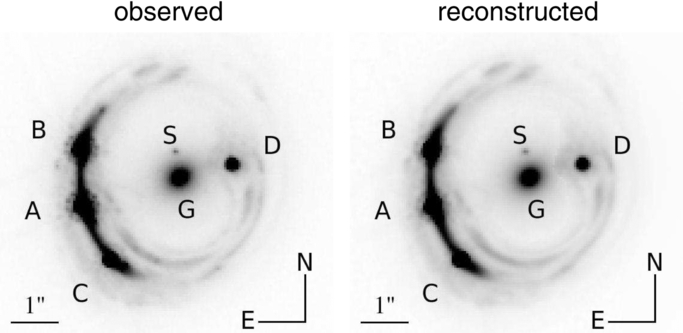
\includegraphics[height=3.5cm]{figures/Suyu14_fig1.jpg}
\caption{Comparison between imaging data available in the nineties
\citep[eft panel, from][]{Sch++97} and in the most recent studies
\citep[middle and right panels, from][]{Suy++14}). With modern data the
structure of the quasar host galaxy can be modeled in great detail,
providing thousands of constraints on the deflection angle, and thus on
the derivatives of the gravitational potential.}
\label{fig:oldvsmodernimage}
\end{figure*}
%%%%%%%%%%%%%%%%%%%%%%%%%%%%%%%%%%%%%%

Ultimately, the controversies over systematic errors were essential to
spur the community to overcome the difficulties and find ways to
address them. This is a natural and probably inevitable part of the
scientific process. However, the bitterness of some of those
controversies during the ninenties and early naughties still resonates
today: unfortunately, some of the scientists that followed the field
with excitement at that time are still under the impression that
strong lensing time delays are inherently inaccurate and imprecise. As
we have briefly described here, and we will show in detail in the
next sections, in the last twenty years the field has moved forward
considerably implementing many solutions to the lessons learned the
hard way.



% % % % % % % % % % % % % % % % % % % % % % % % % % % % % % % % % %

%\subsection{Current context}
%\label{sec:context}

%Towards accurate cosmology with multiple probes.

%Time delays lie between local Hubble constant measurement and other
%kinematic probes at intermediate redshift (BAO, SNe).

%Requirements of each probe: sufficient precision to test
%systematics of the others.

%%%%%%%%%%%%%%%%%%%%%%%%%%%%%%%%%%%%%%%%%%%%%%%%%%%%%%%%%%%%%%%%%%%

\section{Theoretical background [PJM]}
\label{sec:theory}

%Gravitational lensing. Time delay surface. Distance.

%Notes on lens mass distribution.

%Notes on weak lensing effects.

Lensing, Fermat's principle and potential.

FIGURE: SCHEMATIC WAVEFRONT DIAGRAM FROM T\&E15. 

Time delay distance. 

Importance of mass distribution in lens.

Model (mass-sheet) degeneracy and its generalizations

Importance of mass along the line sight - the universe is not Friedmann Lemaitre Robertson Walker.

POSSIBLE FIGURE: ILLUSTRATION OF LINE OF SIGHT EFFECTS? CARTOON COMPARING IDEALIZED UNIVERSE TO OVER/UNDER DENSE LINE OF SIGHT [PJM]

%%%%%%%%%%%%%%%%%%%%%%%%%%%%%%%%%%%%%%%%%%%%%%%%%%%%%%%%%%%%%%%%%%%

\section{Modern Time delay distance measurement 2010+ [PJM]}
\label{sec:timedelay}

%Outline key analysis steps.

%Next three sections will each describe current state of the art,
%current limitations, and principal sources of systematic error
%of the three key parts of the problem.



%%%%%%%%%%%%%%%%%%%%%%%%%%%%%%%%%%%%%%%%%%%%%%%%%%%%%%%%%%%%%%%%%%%

\subsection{Measuring time delays [PJM]}
label{ssec:tdmeasurements}

%Preamble.

Mention importance of blindness in all measurements. 


% % % % % % % % % % % % % % % % % % % % % % % % % % % % % % % % % %

\subsubsection{Monitoring Observations}

%State of the art: COSMOGRAIL optical monitoring.

%Limitations: scheduling.

%Systematic errors: uniform calibration and photometry.

Fassnacht for B1608
COSMOGRAIL.
Others?


% % % % % % % % % % % % % % % % % % % % % % % % % % % % % % % % % %

\subsubsection{Lightcurve Analysis}

%State of the art: TDC results.

%Systematic errors: microlensing, correlated noise.

COSMOGRAIL
TDC


%%%%%%%%%%%%%%%%%%%%%%%%%%%%%%%%%%%%%%%%%%%%%%%%%%%%%%%%%%%%%%%%%%%

\subsection{Modeling the lens mass distribution [TT]}
\label{sec:lensmodel}

%Preamble.

% % % % % % % % % % % % % % % % % % % % % % % % % % % % % % % % % %

\subsubsection{High Resolution Imaging Observations}

%State of the art: HST, Keck AO.

%Limitations: resolution, bright quasar images.


% % % % % % % % % % % % % % % % % % % % % % % % % % % % % % % % % %

\subsubsection{Lens Modeling Techniques}

%State of the art: pixelated source reconstruction,
%simply-parameterised lens mass distributions, MCMC.

%Limitations: skilled labor.

%Systematic errors: source pixelation/regularisation, lens model
%assumptions.

\subsubsection{The Role of Stellar kinematics}


%%%%%%%%%%%%%%%%%%%%%%%%%%%%%%%%%%%%%%%%%%%%%%%%%%%%%%%%%%%%%%%%%%%

\subsection{Lens environments and line of sight effects [PJM]}
\label{sec:los}

%State of the art: ray-traced cosmological simulations, matched via
%number counts.

%Limitations/systematics: incomplete model: local vs line of sight
%mass,  ignoring multi-plane lensing, external convergence only.


%%%%%%%%%%%%%%%%%%%%%%%%%%%%%%%%%%%%%%%%%%%%%%%%%%%%%%%%%%%%%%%%%%%

\section{From time delay distances to cosmography [PJM]}
\label{sec:cosmo}

%Approach: combining CMB and time delay distances. Blinding.

%Results. Internal consistency. Consistency with other probes.


%%%%%%%%%%%%%%%%%%%%%%%%%%%%%%%%%%%%%%%%%%%%%%%%%%%%%%%%%%%%%%%%%%%

\section{Outlook [TT]}
\label{sec:outlook}

%Preamble.

% % % % % % % % % % % % % % % % % % % % % % % % % % % % % % % % % %

\subsection{Precision [PJM}

FIGURE: Forecasts for 10,50,100,1000 lenses for various cosmological models (w, wa+w0, curvature etc etc). CosmoSIS forecasts (ackn. Dave \& Elise, ask them). 

Check Jee et al.

%Sample size. Stage 3, stage 4 surveys. Monitoring solutions.

%Extrapolations to N lenses assuming X\% precision per time delay
%distance, forecasts.

% % % % % % % % % % % % % % % % % % % % % % % % % % % % % % % % % %

\subsection{Accuracy [PJM]}

%Addressing systematics associated with time delay measurement, lens
%modeling, environment characterisation.

%Accuracy in joint analysis: hierarchical inference.

Discussion of systematic uncertainties

Time delay measurement. Light curve quality. 

Lens mass modeling. Percent-level systematics due to model assumptions (ie MSD). IFU observations, resolved stellar kinematics. Ensembles. 

Environment and line of sight

Time delay perturbations (someone's noise is somebody else's signal..)

The importance of blinding.

\subsection{Cosmic complementarity [TT]}

What's the point? Arent' other probes already doing it? Our place in the cosmology ecosystem. Discuss place relative to other distance indicators like Cepheids, BAO, Sne. Then complementarity with growth of structure probes like weak lensing, clusters etc etc. How important is H0?

Importance of multiple INDEPENDENT measurements for discovery of new physics.

%%%%%%%%%%%%%%%%%%%%%%%%%%%%%%%%%%%%%%%%%%%%%%%%%%%%%%%%%%%%%%%%%%%

\section{Summary [TT]}
\label{sec:summary}

%%%%%%%%%%%%%%%%%%%%%%%%%%%%%%%%%%%%%%%%%%%%%%%%%%%%%%%%%%%%%%%%%%%

%\paragraph{Paragraph headings} Use paragraph headings as needed.
%\begin{equation}
%a^2+b^2=c^2
%\end{equation}

% For one-column wide figures use
%\begin{figure}
% Use the relevant command to insert your figure file.
% For example, with the graphicx package use
%  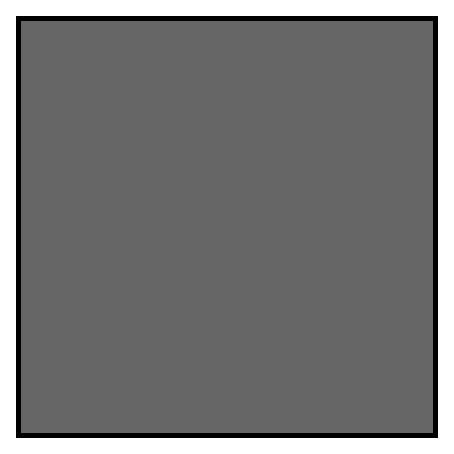
\includegraphics{example.eps}
% figure caption is below the figure
%\caption{Please write your figure caption here}
%\label{fig:1}       % Give a unique label
%\end{figure}
%
% For two-column wide figures use
%\begin{figure*}
% Use the relevant command to insert your figure file.
% For example, with the graphicx package use
%  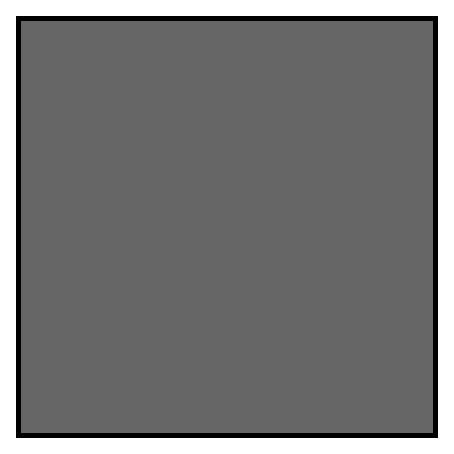
\includegraphics[width=0.75\textwidth]{example.eps}
% figure caption is below the figure
%\caption{Please write your figure caption here}
%\label{fig:2}       % Give a unique label
%\end{figure*}
%
% For tables use
%\begin{table}
% table caption is above the table
%\caption{Please write your table caption here}
%\label{tab:1}       % Give a unique label
% For LaTeX tables use
%\begin{tabular}{lll}
%\hline\noalign{\smallskip}
%first & second & third  \\
%\noalign{\smallskip}\hline\noalign{\smallskip}
%number & number & number \\
%number & number & number \\
%\noalign{\smallskip}\hline
%\end{tabular}
%\end{table}

%%%%%%%%%%%%%%%%%%%%%%%%%%%%%%%%%%%%%%%%%%%%%%%%%%%%%%%%%%%%%%%%%%%

\begin{acknowledgements}
T.T. thanks the Packard Foundation for generous support through a Packard Research Fellowship, the NSF for funding through NSF grant AST-1450141, ``Collaborative Research: Accurate cosmology with strong gravitational lens time delays''.	
Thank people who give comments/input. Thank funding agencies.
\end{acknowledgements}

%%%%%%%%%%%%%%%%%%%%%%%%%%%%%%%%%%%%%%%%%%%%%%%%%%%%%%%%%%%%%%%%%%%

% BibTeX users please use one of
%\bibliographystyle{spbasic}      % basic style, author-year citations
%\bibliographystyle{spmpsci}      % mathematics and physical sciences
\bibliographystyle{spphys}       % APS-like style for physics
\bibliography{references}   % name your BibTeX data base

% Non-BibTeX users please use
%\begin{thebibliography}{}
%
% and use \bibitem to create references. Consult the Instructions
% for authors for reference list style.
%
%\bibitem{RefJ}
% Format for Journal Reference
%Author, Article title, Journal, Volume, page numbers (year)
% Format for books
%\bibitem{RefB}
%Author, Book title, page numbers. Publisher, place (year)
% etc
%\end{thebibliography}

%%%%%%%%%%%%%%%%%%%%%%%%%%%%%%%%%%%%%%%%%%%%%%%%%%%%%%%%%%%%%%%%%%%

\end{document}

%%%%%%%%%%%%%%%%%%%%%%%%%%%%%%%%%%%%%%%%%%%%%%%%%%%%%%%%%%%%%%%%%%%
